\begin{figure}[htbp]
	\centering
	\begin{tikzpicture}

		\node(rpi){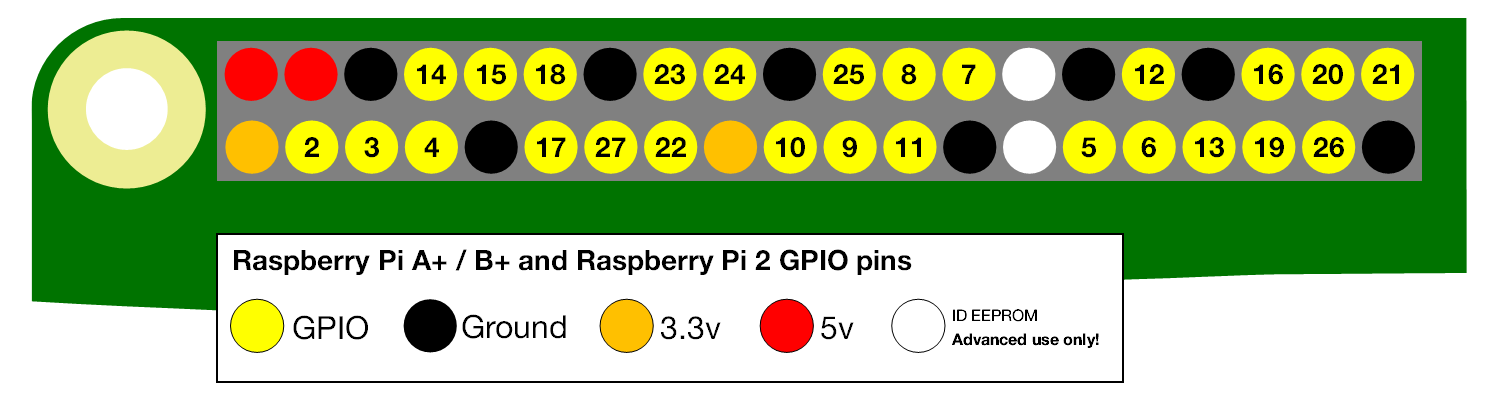
\includegraphics[width=0.5\textwidth,trim={0 6cm 0 0},clip]{./figures/gpio.png}};
		\node[above=15mm of rpi,xshift=-1.2cm](sonar){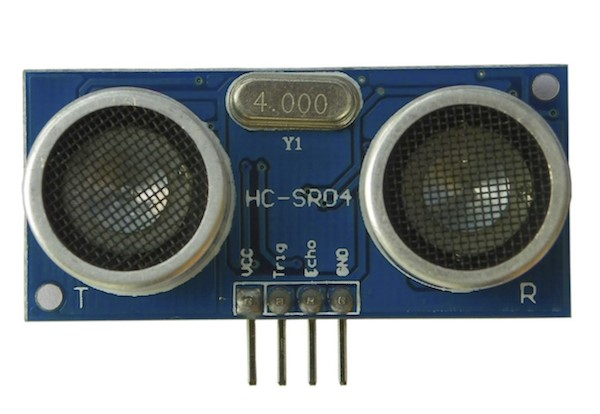
\includegraphics[width=0.3\textwidth,trim={0 2mm 0 2mm},clip]{./figures/hc-sr04.jpg}};

		\coordinate(VCC) at ($(sonar.south)+(-3.8mm,5mm)$);
		\coordinate(TRIG) at ($(sonar.south)+(-1.5mm,5mm)$);
		\coordinate(ECHO) at ($(sonar.south)+(1mm,5mm)$);
		\coordinate(GND) at ($(sonar.south)+(3.3mm,5mm)$);

		\coordinate(v) at ($(sonar.south)+(-3.8mm,0)$);
		\coordinate(t) at ($(sonar.south)+(-1.5mm,-2mm)$);
		\coordinate(e) at ($(sonar.south)+(1mm,-7mm)$);
		\coordinate(g) at ($(sonar.south)+(3.3mm,-15mm)$);

		\coordinate(vcc) at ($(rpi.north west)+(17.6mm,-5.7mm)$);
		\coordinate(gnd) at ($(rpi.north west)+(20.8mm,-5.7mm)$);
		\coordinate(trig) at ($(rpi.north west)+(24.0mm,-5mm)$);
		\coordinate(echo) at ($(rpi.north west)+(27.0mm,-5mm)$);

		\node[draw,fill=white,minimum width=2mm,minimum height=5mm,inner sep=0,above=2mm of e](r1){\tiny R$_1$};
		\node[draw,fill=white,minimum width=2mm,minimum height=5mm,inner sep=0,above=7mm of gnd](r2){\tiny R$_2$};

		\draw[line width=0.5mm,blue!50] (e) -| (r2);
		\draw[line width=0.5mm,blue!50] (r2) -- (gnd);

		\draw[line width=0.5mm,red] (VCC) -- (v) -| (vcc);
		\draw[line width=0.5mm,black] (GND) -- (g) -| (gnd);
		\draw[line width=0.5mm,green!80] (TRIG) -- (t) -| (trig);
		\draw[line width=0.5mm,blue!80] (ECHO) -- (r1);
		\draw[line width=0.5mm,blue!80] (r1) -- (e) -| (echo);
		
		\node[fill=blue!80,circle,inner sep=0.4mm,above=12.3mm of echo] (connEcho){};
		\node[fill=black,circle,inner sep=0.4mm,above=5mm of gnd] (connGnd){};

	\end{tikzpicture}
	\caption{Connection of the HC-SR04 sensor to the Raspberry Pi}
	\label{fig:sonarconnect}
\end{figure}
